\documentclass[main.tex]{subfiles}
\begin{document}

\section{Introduction}
\label{sec:intro}
%Describe the generation of timing/synchronisation signals and and distribution to the detectors.
The primary functions of the \dword{dts} are to provide a stable and phase-aligned master clock to all DAQ components; receive external signals, which may include triggers, into the DUNE clock domain and time-stamp them; distribute synchronization, calibration, and potentially trigger commands to the DAQ system; perform continuous self-checking; and provide status information to the DUNE \dword{ccm}. In addition, the timing system acts as a data source, providing a record of timing signals received, distributed, or throttled. The goals of the \dword{dune} physics programme impose the following synchronisation requirements:

\begin{itemize}
    \item synchronisation between components of a \dword{detmodule} of $\mathcal{O}(\SI{5}{\ns})$
    \item synchronisation between \dword{dts} timestamp and \dword{tai} of $\mathcal{O}(\SI{1}{ms})$.
\end{itemize}

%Due to different development histories of the \dword{bde} and \dword{tde} technologies of the \dword{vd} \dword{detmodule}, different timing systems are used for each one. The \dword{vd} \dword{bde}, as well as the entirety of the \dword{hd} \dword{detmodule} make use of the \dword{dts}. The protocol is based around a 8b/10b encoded serial data stream, and it distributes a \SI{62.5}{\MHz} clock to \dword{hd} and \dword{vd} \dword{bde} endpoints. The \dword{vd} \dword{tde} are synchronised via a \dword{wr} network \cite{wr_ohwr}, which uses a \SI{125}{\MHz} clock. The \dword{wrgm} of the \dword{vd} \dword{tde} \dword{wr} network will be driven by a \SI{10}{\MHz} clock and \dword{pps} provided by a specialised \dword{dts} endpoint.

This document describes the design of the \dword{dts}, including internal interfaces between the different components of the system. 

%The external endpoint interface and \dword{dts} communication protocol are described in a separate document \cite{dts_sp_protocol}. This is also true for the design of the firmware which will be running in the different components of the system, and the software which will be used to control and monitor the \dword{dts} \cite{dts_sp_firmware}  \cite{dts_sp_software}.

\section{DUNE Timing System design}
\label{sec:system_design}
\subsection{Overview}
A custom electronics module, the \dword{gib} receives a high-quality \SI{10}{\MHz} clock, provided by a \dword{gpsdo}. The \dword{gib} also receives a serial \dword{irig} signal \cite{irig}, which has \dword{tai} encoded within it. Both the GPS receiver and the \dword{gib} are envisaged to be located on the surface. The \dword{gib} generates the \dword{dts} timestamp and encodes it into periodic synchronisation messages. These messages are transmitted to each \dword{detmodule} over a single mode optical fibre, using the \dword{dts} protocol. The \SI{62.5}{\MHz} clock is embedded within the data stream.

The data stream at each \dword{detmodule} is received, and decoded into separate clock and data signals by a \dword{mib}, which is hosted in a \dword{utca} crate. The \dword{mib} multiplexes synchronization and other timing messages, along with user-defined message sequences generated by software, into a single data stream. 

The \dword{mib} distributes the recovered clock and the data stream to the \dwords{amc}, also hosted in the same \dword{utca} crate. The clock and timing data are fanned out to the \dwords{amc} over the \dword{utca} backplane. The \dwords{amc} are the carriers of the \dwords{fib}, which are \dwords{fmc}. The \dwords{fib} are used to broadcast the timing data stream to each timing endpoint, using single mode optical fibres. Each \dword{fib} has eight \dword{sfp} transceiver modules. A \dword{utca} crate can host up to 12 \dwords{amc} for a total of 96 \dword{sfp} interfaces. An \dword{sfp} serves two \dwords{apa}, through the use of an 1:4 optical splitter/combiner (assuming two fibres per \dword{apa}). Some \dwords{sfp} are connected directly to units which interface with external signals (for example, calibration inputs). These \dword{hsi} units contain a timing endpoint, which receives clock and synchronization signals, used to timestamp the external hardware signals.

The serial timing data stream is decoded at each endpoint into separate clock and data signals. A uniform phase-aligned cycle counter, updating at the \dword{dts} frequency of \SI{62.5}{\MHz}, is maintained at all endpoints, allowing commands to take effect simultaneously at all endpoints regardless of cable lengths or other phase delays. Figure \ref{fig:daq-readout-timing} shows the overall arrangement of components within the \dword{dts}.

\begin{figure}[h]
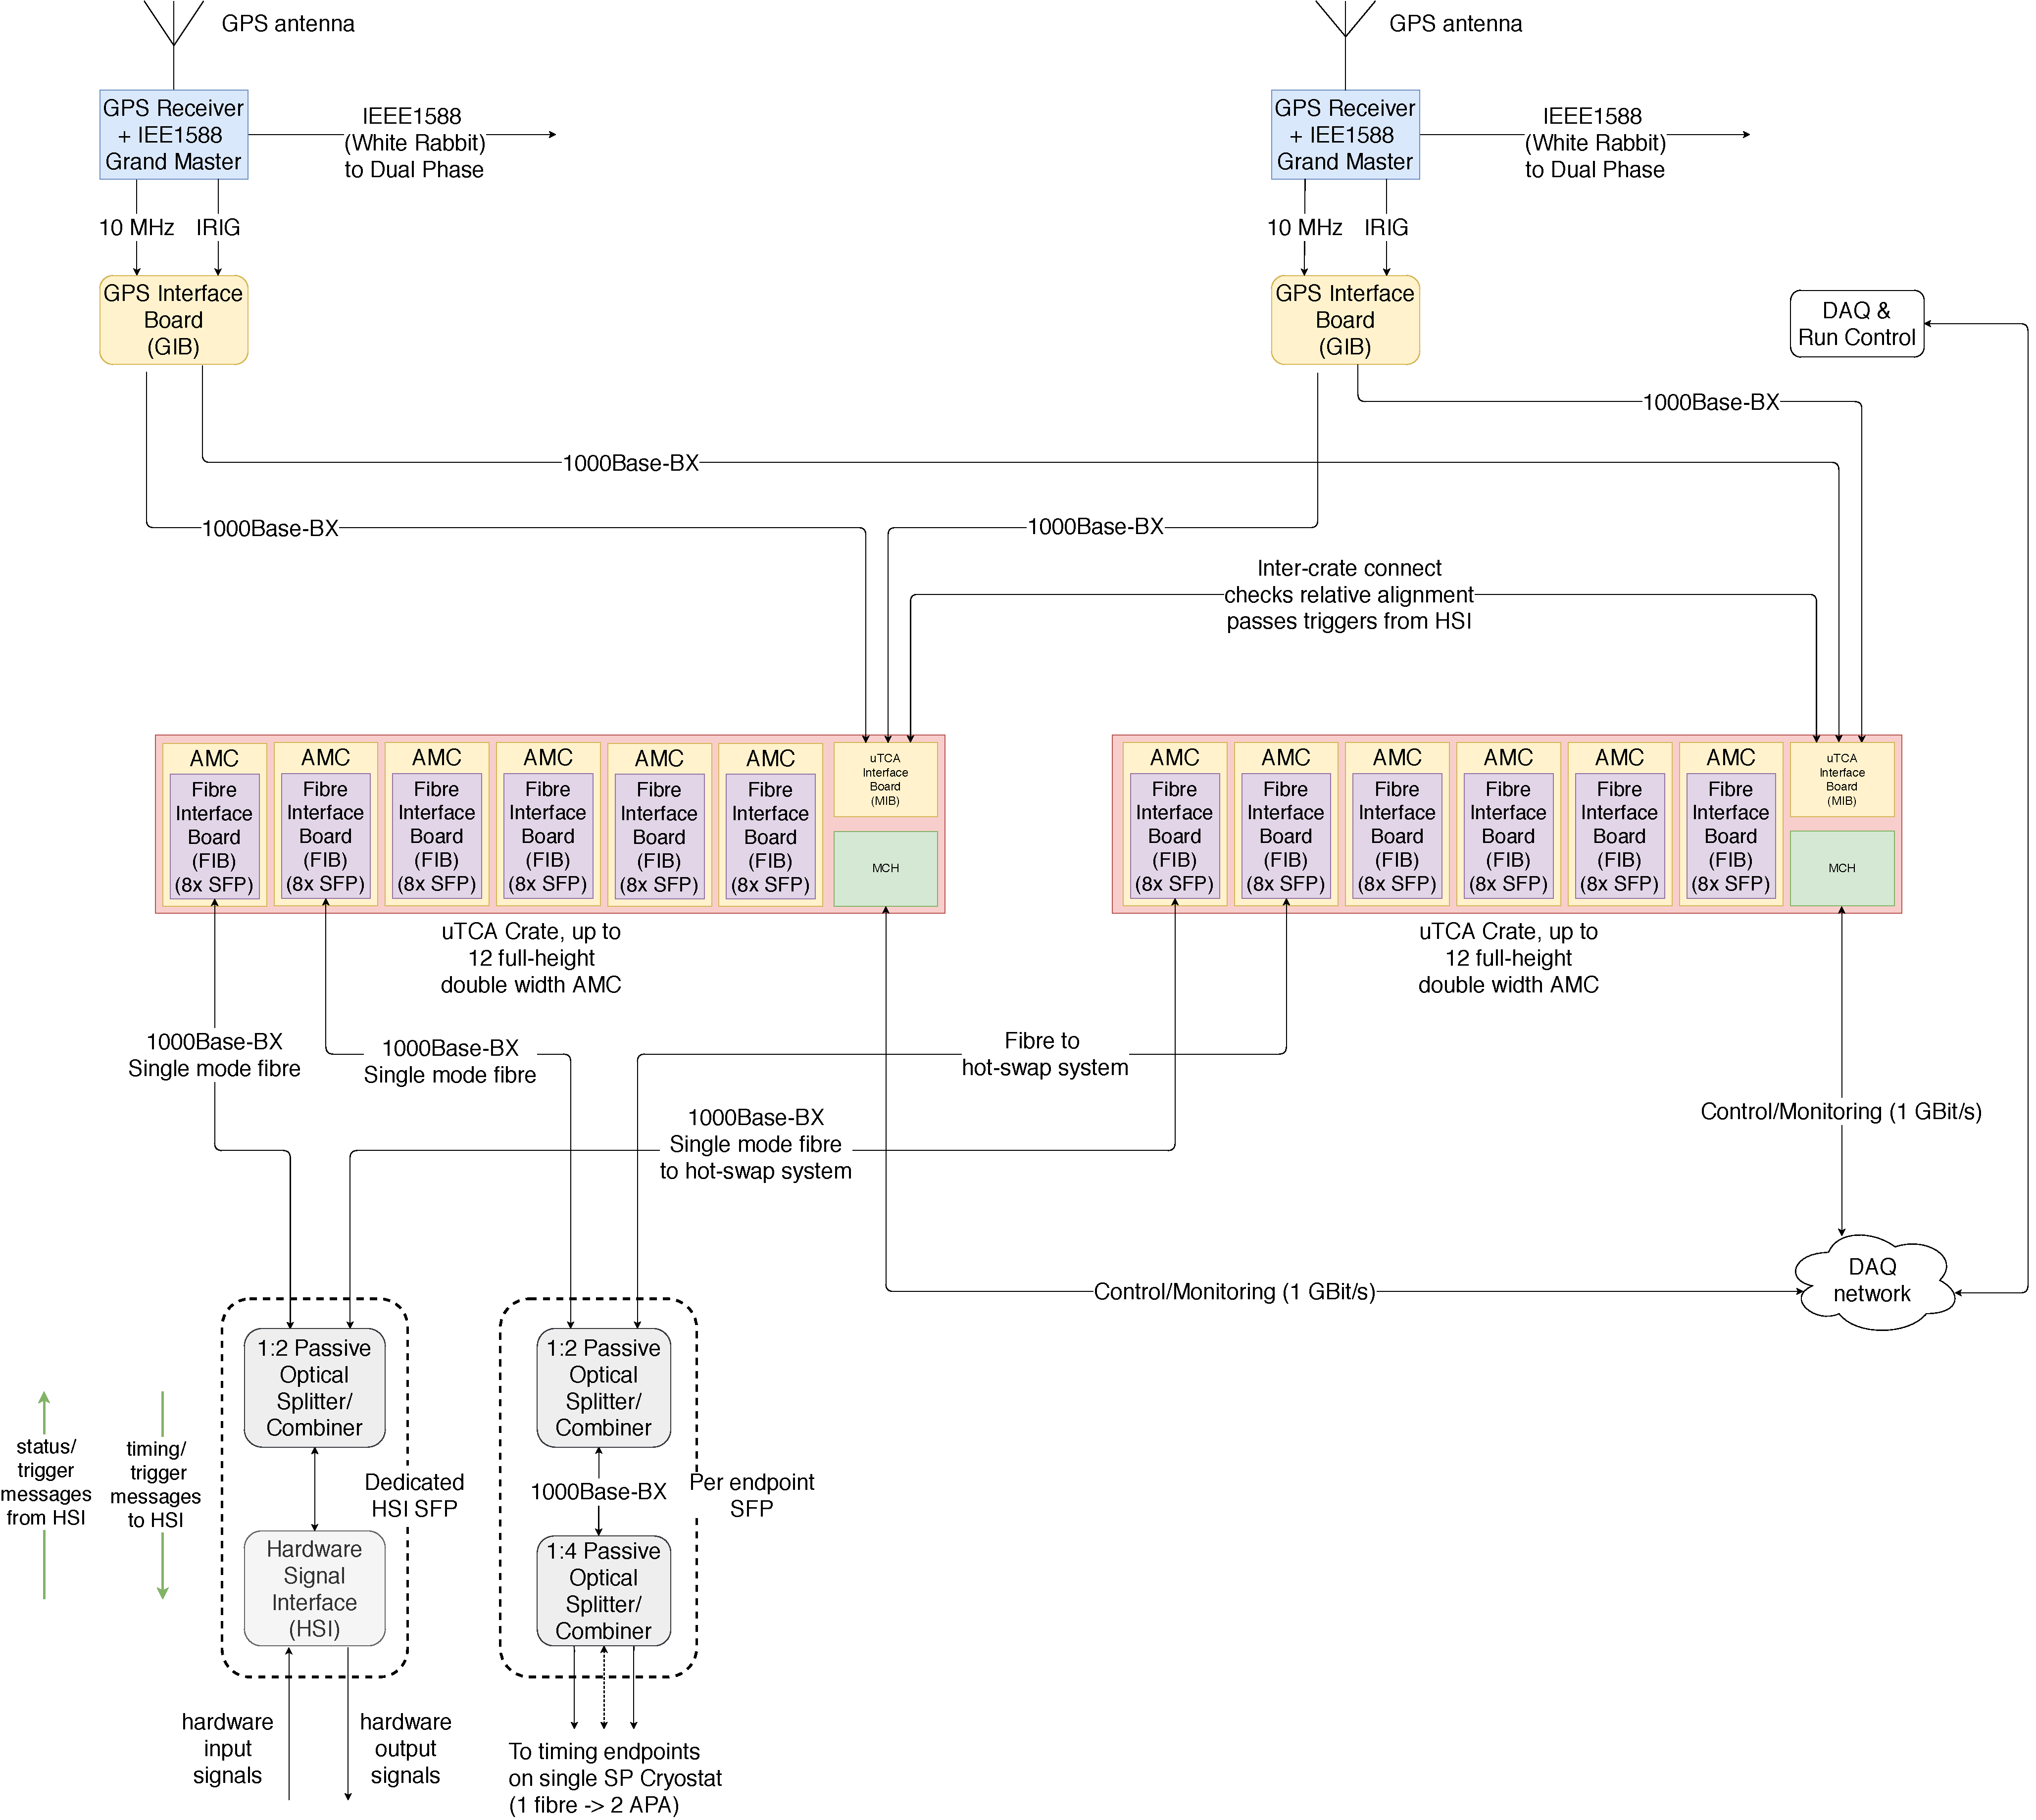
\includegraphics[width=\textwidth]{DUNE_SP_Timing_DAQ_on_CryoM_GPS_In_CUC_01april20.pdf}
\caption{Illustration of the \dword{dts} components for one \dword{sp} \dword{detmodule}.}
\label{fig:daq-readout-timing}
\end{figure}

In order to provide redundancy, and also the ability to easily detect issues with the timing path, two independent GPS systems, i.e. GPS receiver+\dword{gib}, are used. One with an antenna at the head of the Yates Shaft, the other with an antenna at the head of the Ross Shaft. The two independent timing paths are brought to each module cavern, where they both feed two independent redundant \dword{utca} crates, each equipped with a \dword{mib} and a set of \dword{amc}+\dword{fib} pairs. Using 2:1 fibre combiner/splitters, one \dword{dts} unit can be left as a hot spare while the other is active. This also allows testing of new firmware and software during commissioning without the risk of losing the \dword{dts} if a bug is introduced. A \dword{utca} crate interconnect is used to cross-check the two independent timing paths. This, along with thorough system monitoring and an interface to the DUNE \dword{ccm}, will help ensure that the two \dword{dts} crates do not interfere with one another.

\subsection{GPS receiver}
In order to meet the synchronisation requirements outlined in section \ref{sec:intro}, the \dword{dts} needs a stable timing reference from which to generate its \SI{62.5}{\MHz} clock. The reference clock must have both excellent short and long term stability. Such a clock is provided by a \dword{gpsdo}, which works by locking the output of a high quality quartz crystal or rubidium oscillator to a GPS signal. A \dword{gpsdo} combines the long term stability of a GPS signal, with the short term stability (i.e. low jitter) of a free running oscillator. A GPS signal can also be used to provide an absolute time reference, as GPS time is locked to \dword{tai} and \dword{utc}. The time from the GPS signal will be used to initialise and cross-check the timestamp provided by the \dword{dts}.

The \dword{dts} is envisaged to use the SecureSync Time and Frequency Synchronization System \cite{secure_sync_datasheet} as its GPS receiver. The SecureSync system provides a \SI{10}{\MHz} clock generated by a \dword{gpsdo}. The GPS time signal will be output by a dedicated SecureSync module \cite{secure_sync_modules} using an IRIG time code \cite{irig}. IRIG time codes are a standardised format of transmitting timing information. The \SI{10}{\MHz} clock and \dword{irig} data stream will be transmitted to the \dword{gib} using BNC connections. The two physical units are envisaged to be close to each other physically, either in the same or adjacent computing racks. This means that the length of the cables connecting the two devices will not exceed a few metres.

\subsection{DUNE Timing System Protocol}

\subsubsection{Low Level Protocol}

The DUNE Timing System uses duty cycle shift keyed (\dword{dcsk}) with 8b10b encoding as a low level protocol.  \dword{dcsk} gives a rising edge transition at the edge of every unit interval which allows a PLL based clock generator to recover the clock (without the need of a separate Clock and Data Recovery (CDR) device. The 8b10b encoding gives DC-balance which allows an AC-coupled link to be used. Timing data are continuously transmitted at a rate of 62.5Mbit/s. A duty cycle of 25\%/75\% is used to represent 0/1. The 62.5Mbit/s data stream is produced by FPGA and re-timed with a \SI{250}{MHz} , i.e. $4 \times \SI{62.5}{\MHz}$, low-jitter clock. More details are given in \cite{2210.15517}. 

\subsubsection{High Level Protocol}

Timing data are continuously transmitted from the master to each timing endpoint. When commanded the endpoint will transmit data back to the timing master. More details of the high level protocol are given in \cite{ref:dts_high_level_protocol}.

\subsection{GPS Interface Board}
The \dword{gib} receives the \SI{10}{\MHz} reference from the GPS receiver, and uses it to generate the \SI{62.5}{\MHz} \dword{dts} clock. The clock is generated using a high performance jitter-reducing clock generator, providing excellent jitter performance. The IRIG time code is decoded by the \dword{gib} FPGA, and used to initialise the \dword{dts} timestamp. After initialisation, the \dword{dts} timestamp is maintained by the \dword{gib} firmware, where it is continuously updated using the \SI{62.5}{\MHz} clock. The firmware also continuously monitors and records, the relationship between \dword{tai} and the \dword{dts} timestamp.

Synchronisation messages, containing the \dword{dts} timestamp, are generated by the \dword{gib} and transmitted to the \dwords{mib} using the \dword{dts} protocol over single mode optical fibres. Before transmission, the 8b/10b encoded \dword{dts} data stream is re-clocked using a high-speed D flip-flop running at \SI{250}{\MHz}. The \SI{250}{\MHz} clock is derived from the same reference as the \dword{dts} clock, and is generated by the same IC.

The bidirectional optical fibre link to the \dword{mib} is carried on a single-mode fibre using 1000Base-BX \dwords{sfp}, where the outgoing and incoming signals are transmitted using different wavelengths; transmitting happens at \SI{1310}{nm}, whereas receiving is at \SI{1550}{nm}. The return data path will be used to measure the time delay between the \dword{gib} and the \dword{mib}, allowing the \dword{dts} to compensate for it. Both downstream and upstream data make use of the \dword{dts} protocol. Each \dword{gib} will need connect to two \dwords{mib} per \dword{spmod}. Since the \dword{gib} will be on the surface, and the \dword{mib} underground, the optical cables will be several km long.

The logical layout of the \dword{gib} is shown in figure \ref{fig:gib_layout}. Control and management of the \dword{gib} and GPS receiver will be done using a GBit/s Ethernet link and IPBus \cite{ipbus}.

\begin{figure}[h]
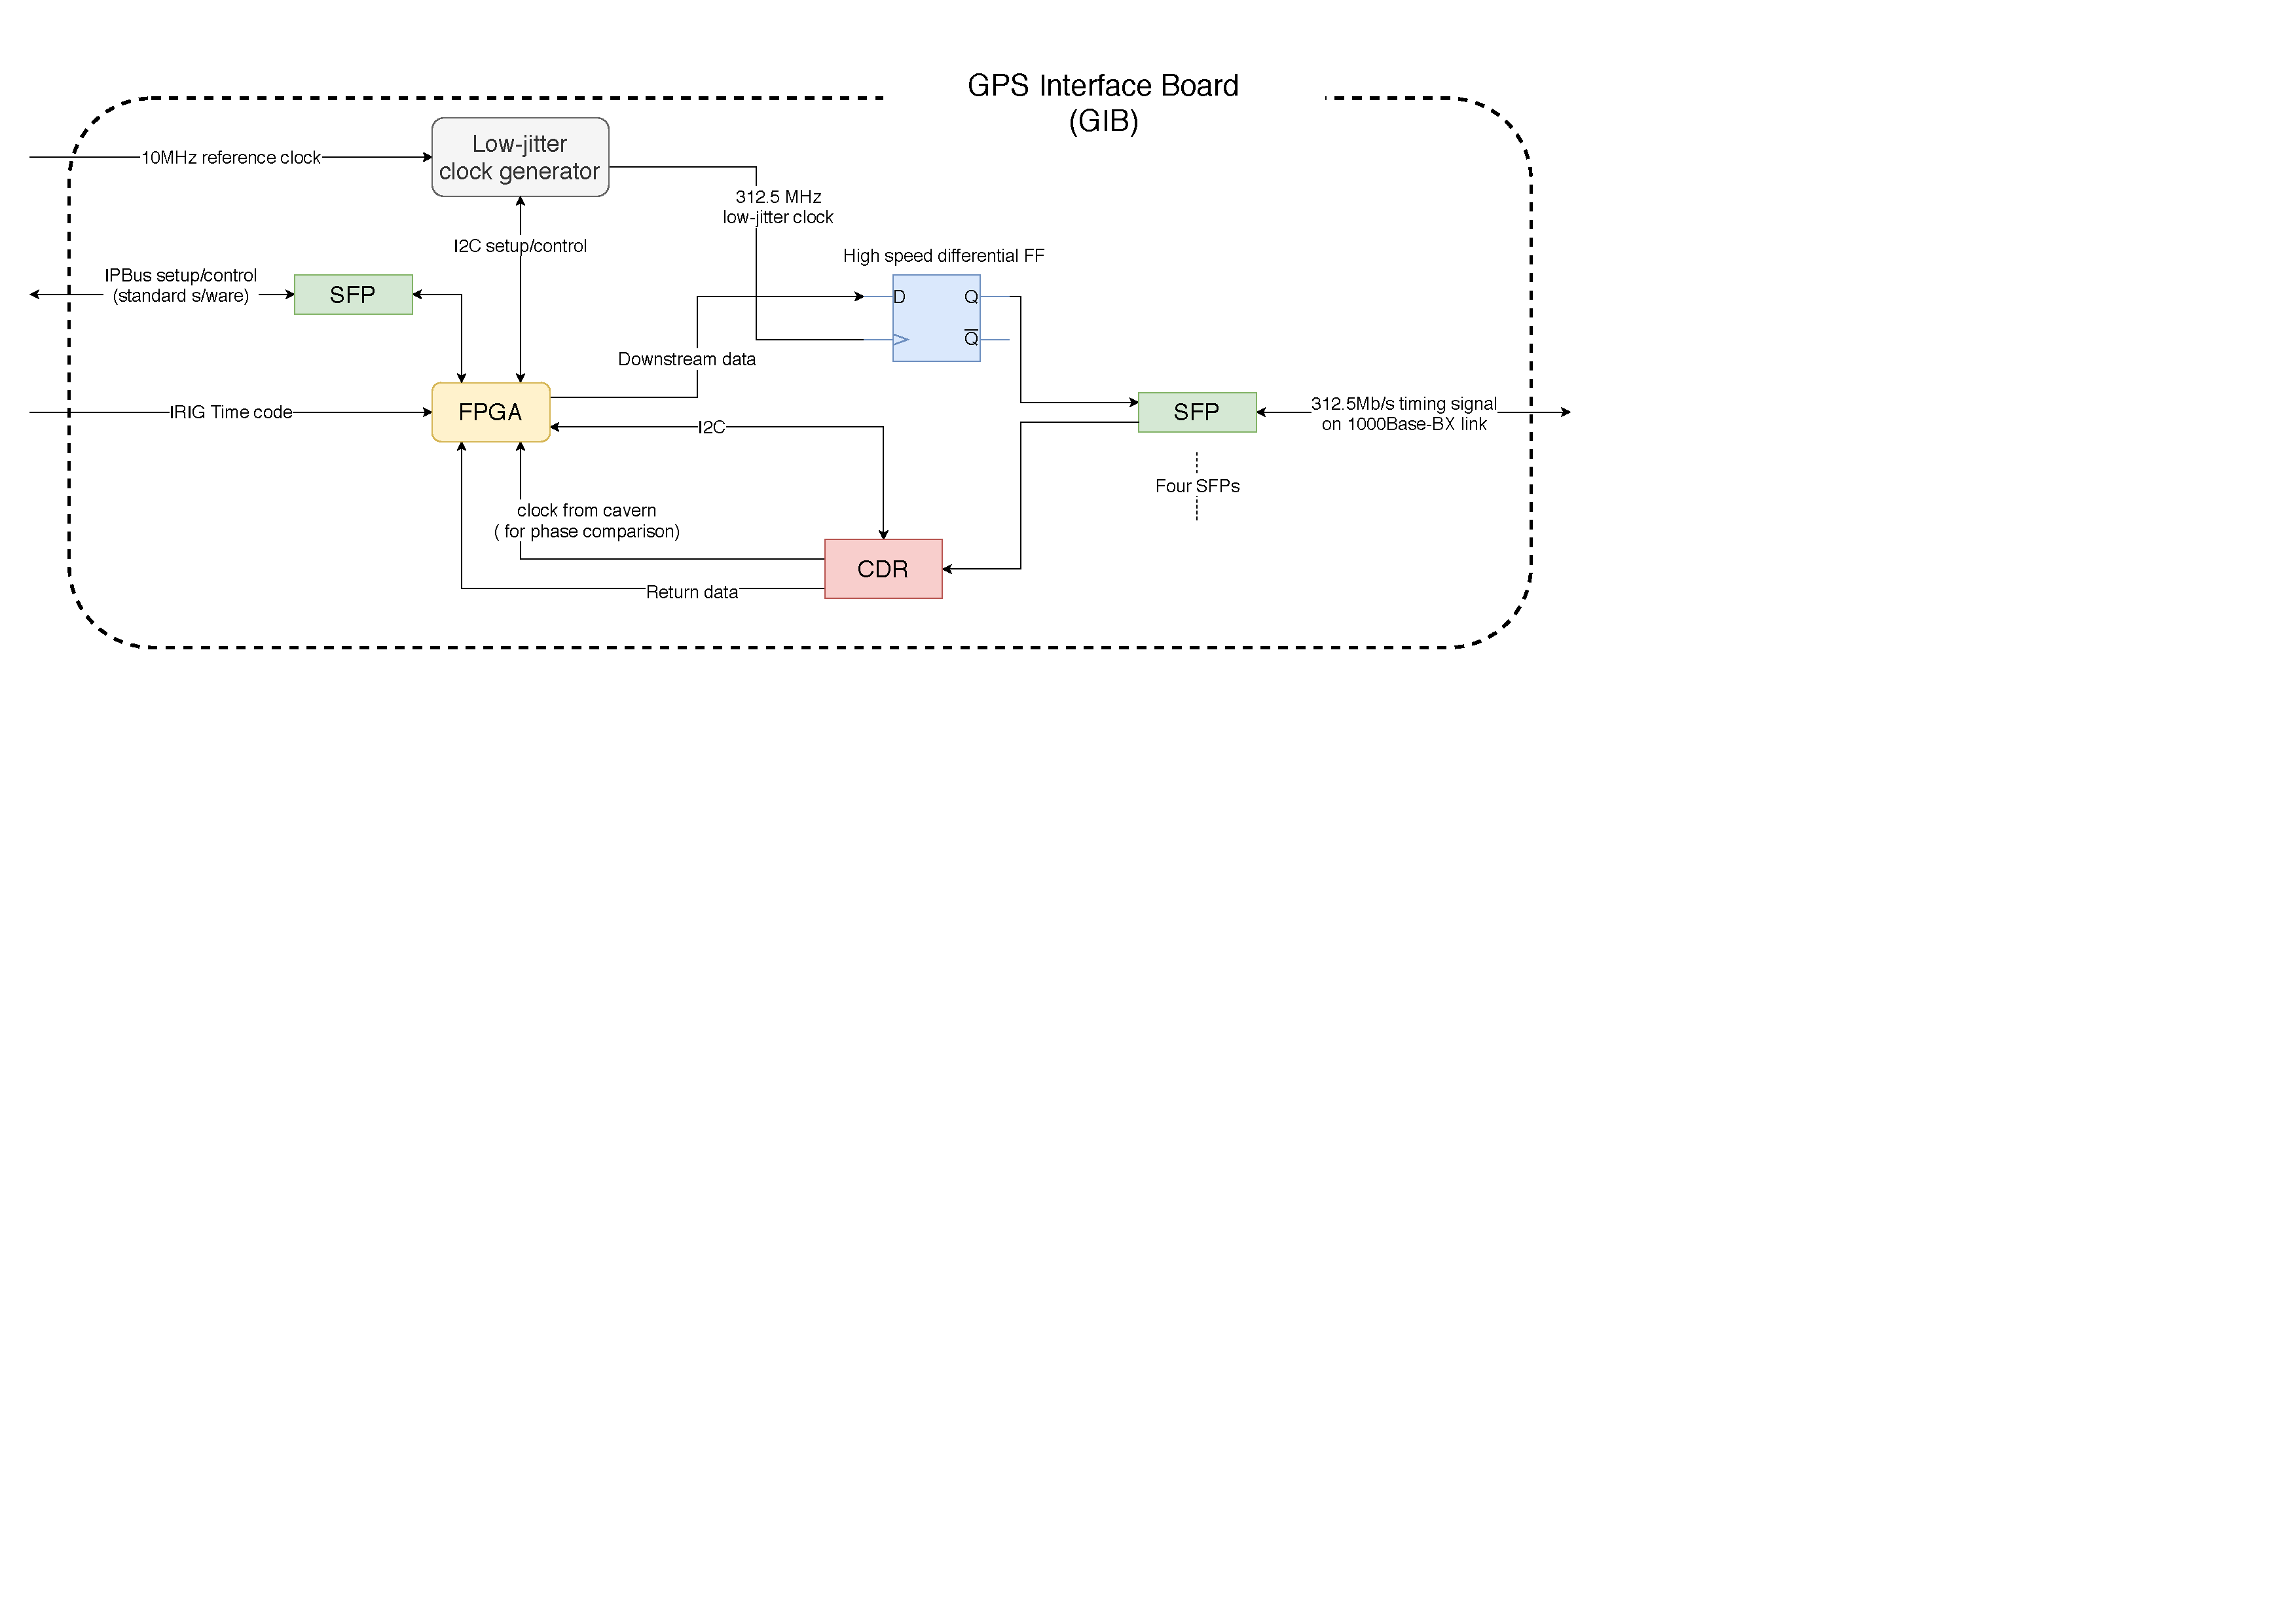
\includegraphics[width=\textwidth]{gib_block_diagram.pdf}
\caption{Illustration of the components in the \dword{gib}.}
\label{fig:gib_layout}
\end{figure}

\subsection[$\mu$TCA Interface Board]{$\boldsymbol{\mu}$TCA Interface Board}
The \dword{mib} receives the \dword{dts} data stream from the \dword{gib} and decodes it into separate clock and data signals using a firmware \dword{cdr} module (a  . The recovered clock is fed into a low jitter clock generator chip to regenerate the \SI{250}{\MHz} clock. The regenerated clock is fanned out to the \dwords{amc} over the \dword{utca} backplane using a clock fan-out chip. The recovered data is sent directly into the \dword{mib} FPGA. The upstream data stream, i.e. from the \dword{mib} to the \dword{gib}, is re-clocked using the low jitter \SI{250}{\MHz} clock, before being sent out over the optical fibre.

The \dword{mib} will sit in the primary \dword{mch} slot of the \dword{utca} crate, and will use three point-to-point LVDS lines to transmit and receive timing data from the \dwords{amc}. The connections are provided by the \dword{utca} backplane. The CLK1 and CLK2 lines from the \dword{mib} are routed to FCLKA and TCLKA on each \dwords{amc}. These lines will be used to transmit the \SI{250}{\MHz} clock and \dword{dts} data stream respectively. TCLKB from each \dwords{amc} is routed to CLK3 on the \dword{mib}, and will be used a return data path back to the \dword{mib}. The interface to the DUNE DAQ and \dword{ccm} systems will be implemented over GBit/s Ethernet and IPBus \cite{ipbus}. The \dword{utca} backplane will provide an Ethernet connection between the \dword{mib} and the actual \dword{mch}, residing in the secondary \dword{mch} slot, which in this case, acts as an Ethernet switch. An illustration of the different \dword{mib} components is shown in figure \ref{fig:mib_layout}. An illustration of the connections inside the \dword{utca}, and the connections to the \dword{hsi} is shown in figure \ref{fig:mib_utca_connections}.

\begin{figure}[h]
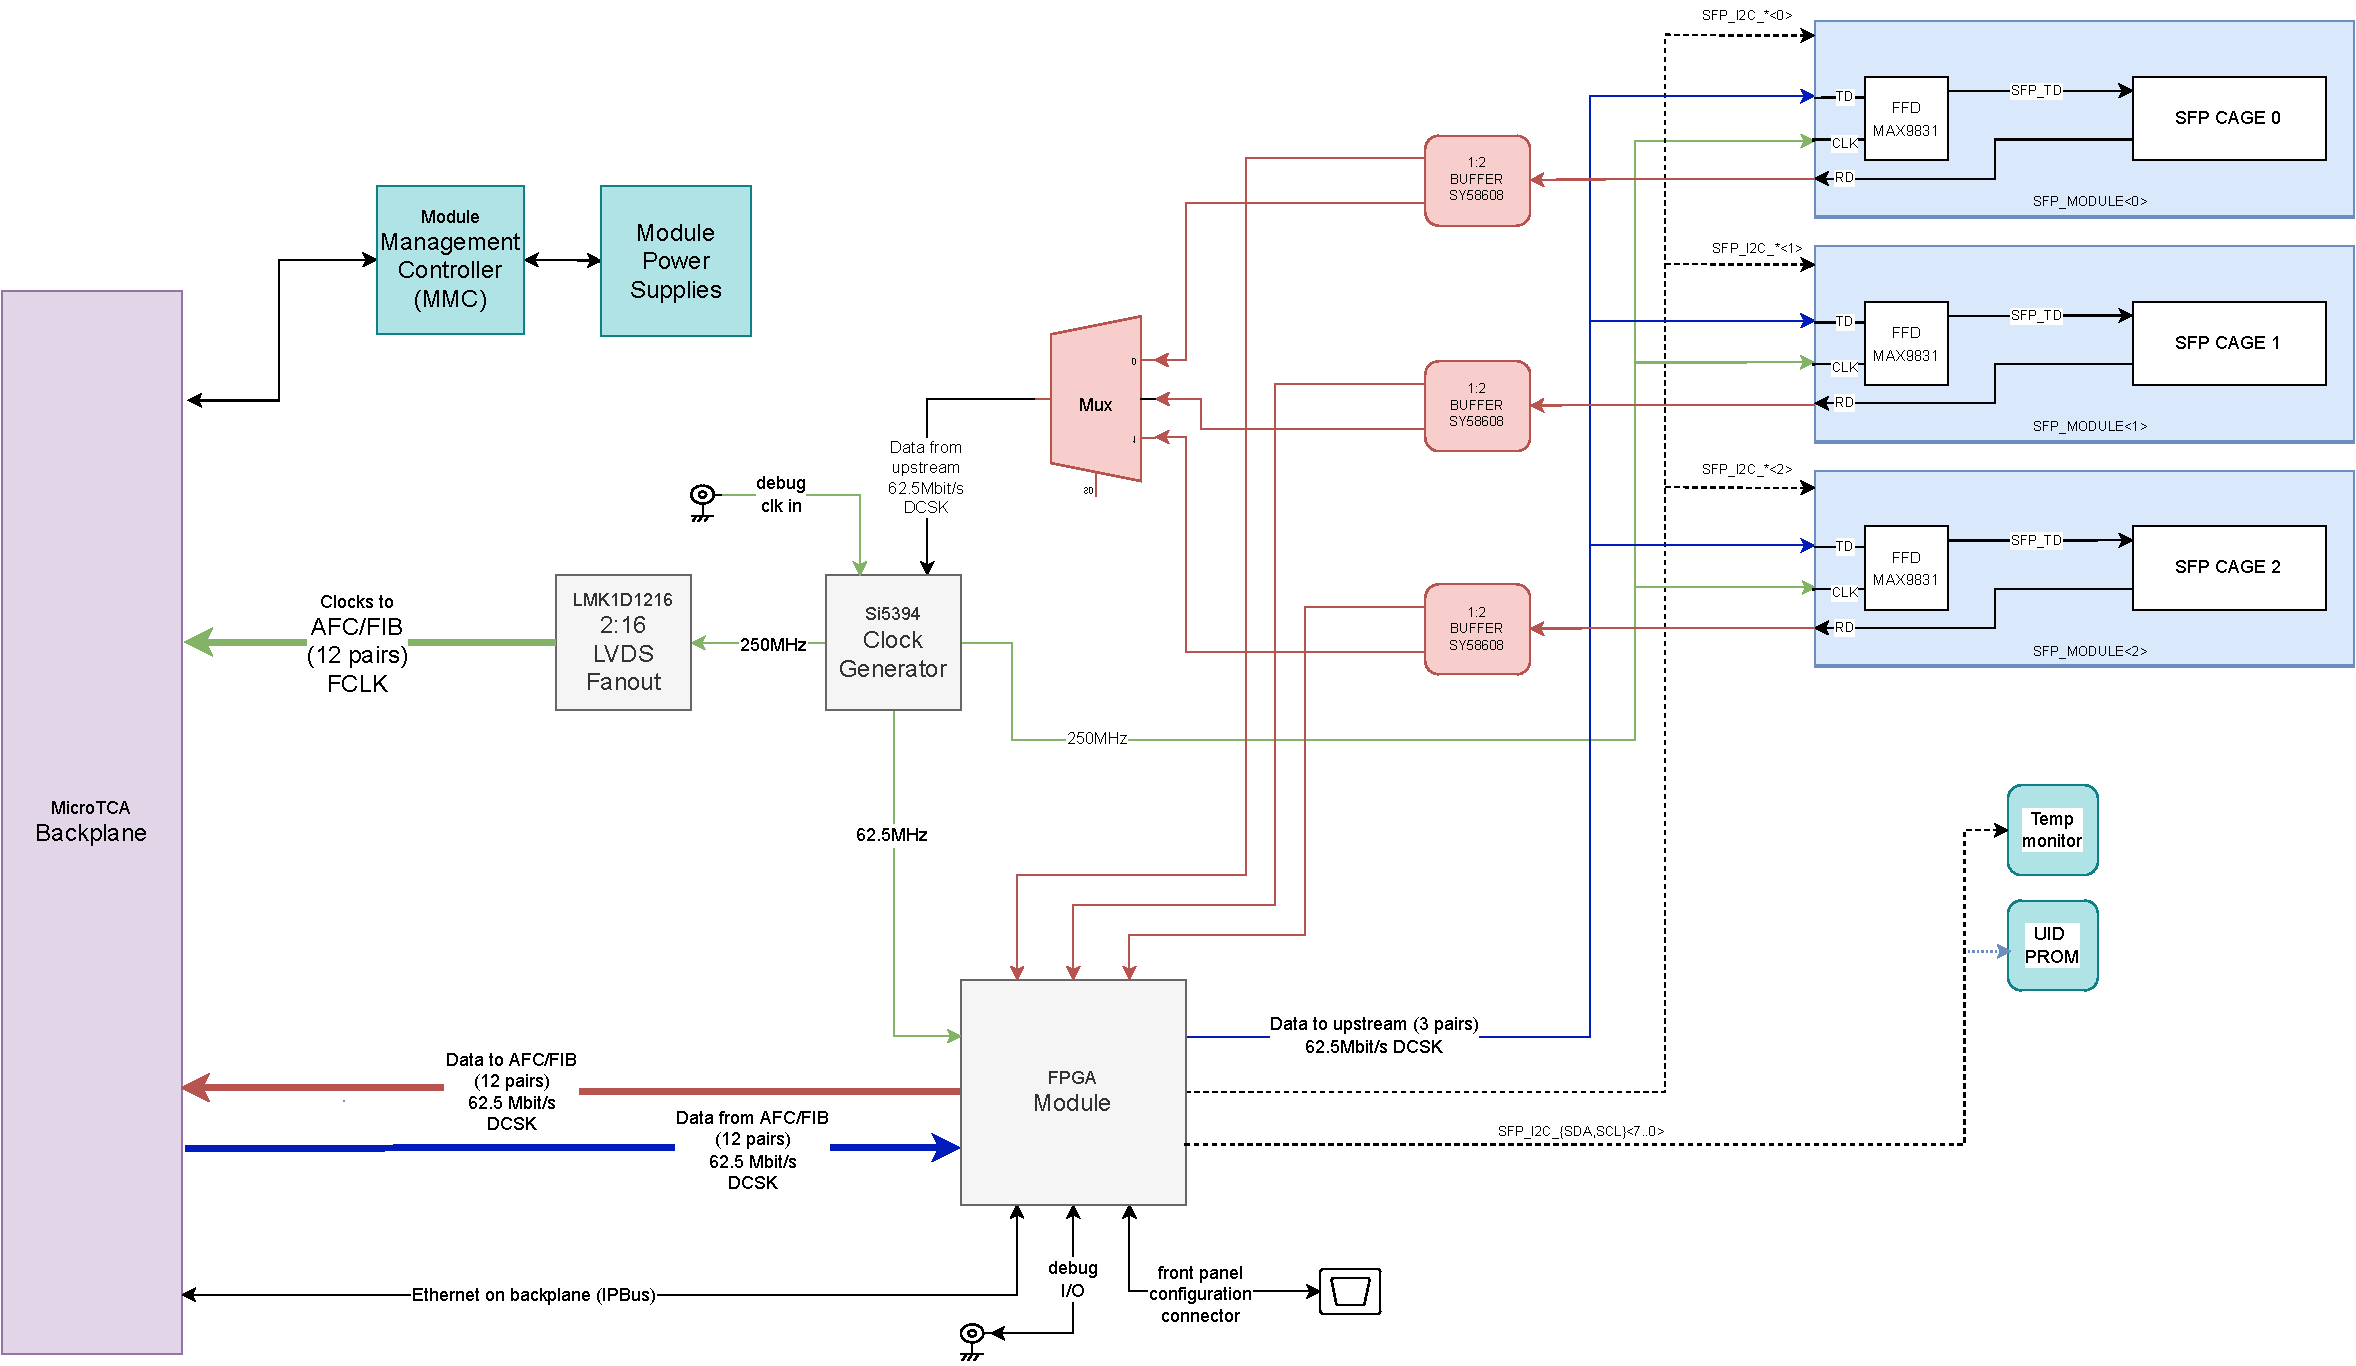
\includegraphics[width=\textwidth]{dune_mib_v2.drawio.pdf}
\caption{Illustration of the components in the \dword{mib}.}
\label{fig:mib_layout}
\end{figure}

\begin{figure}[h]
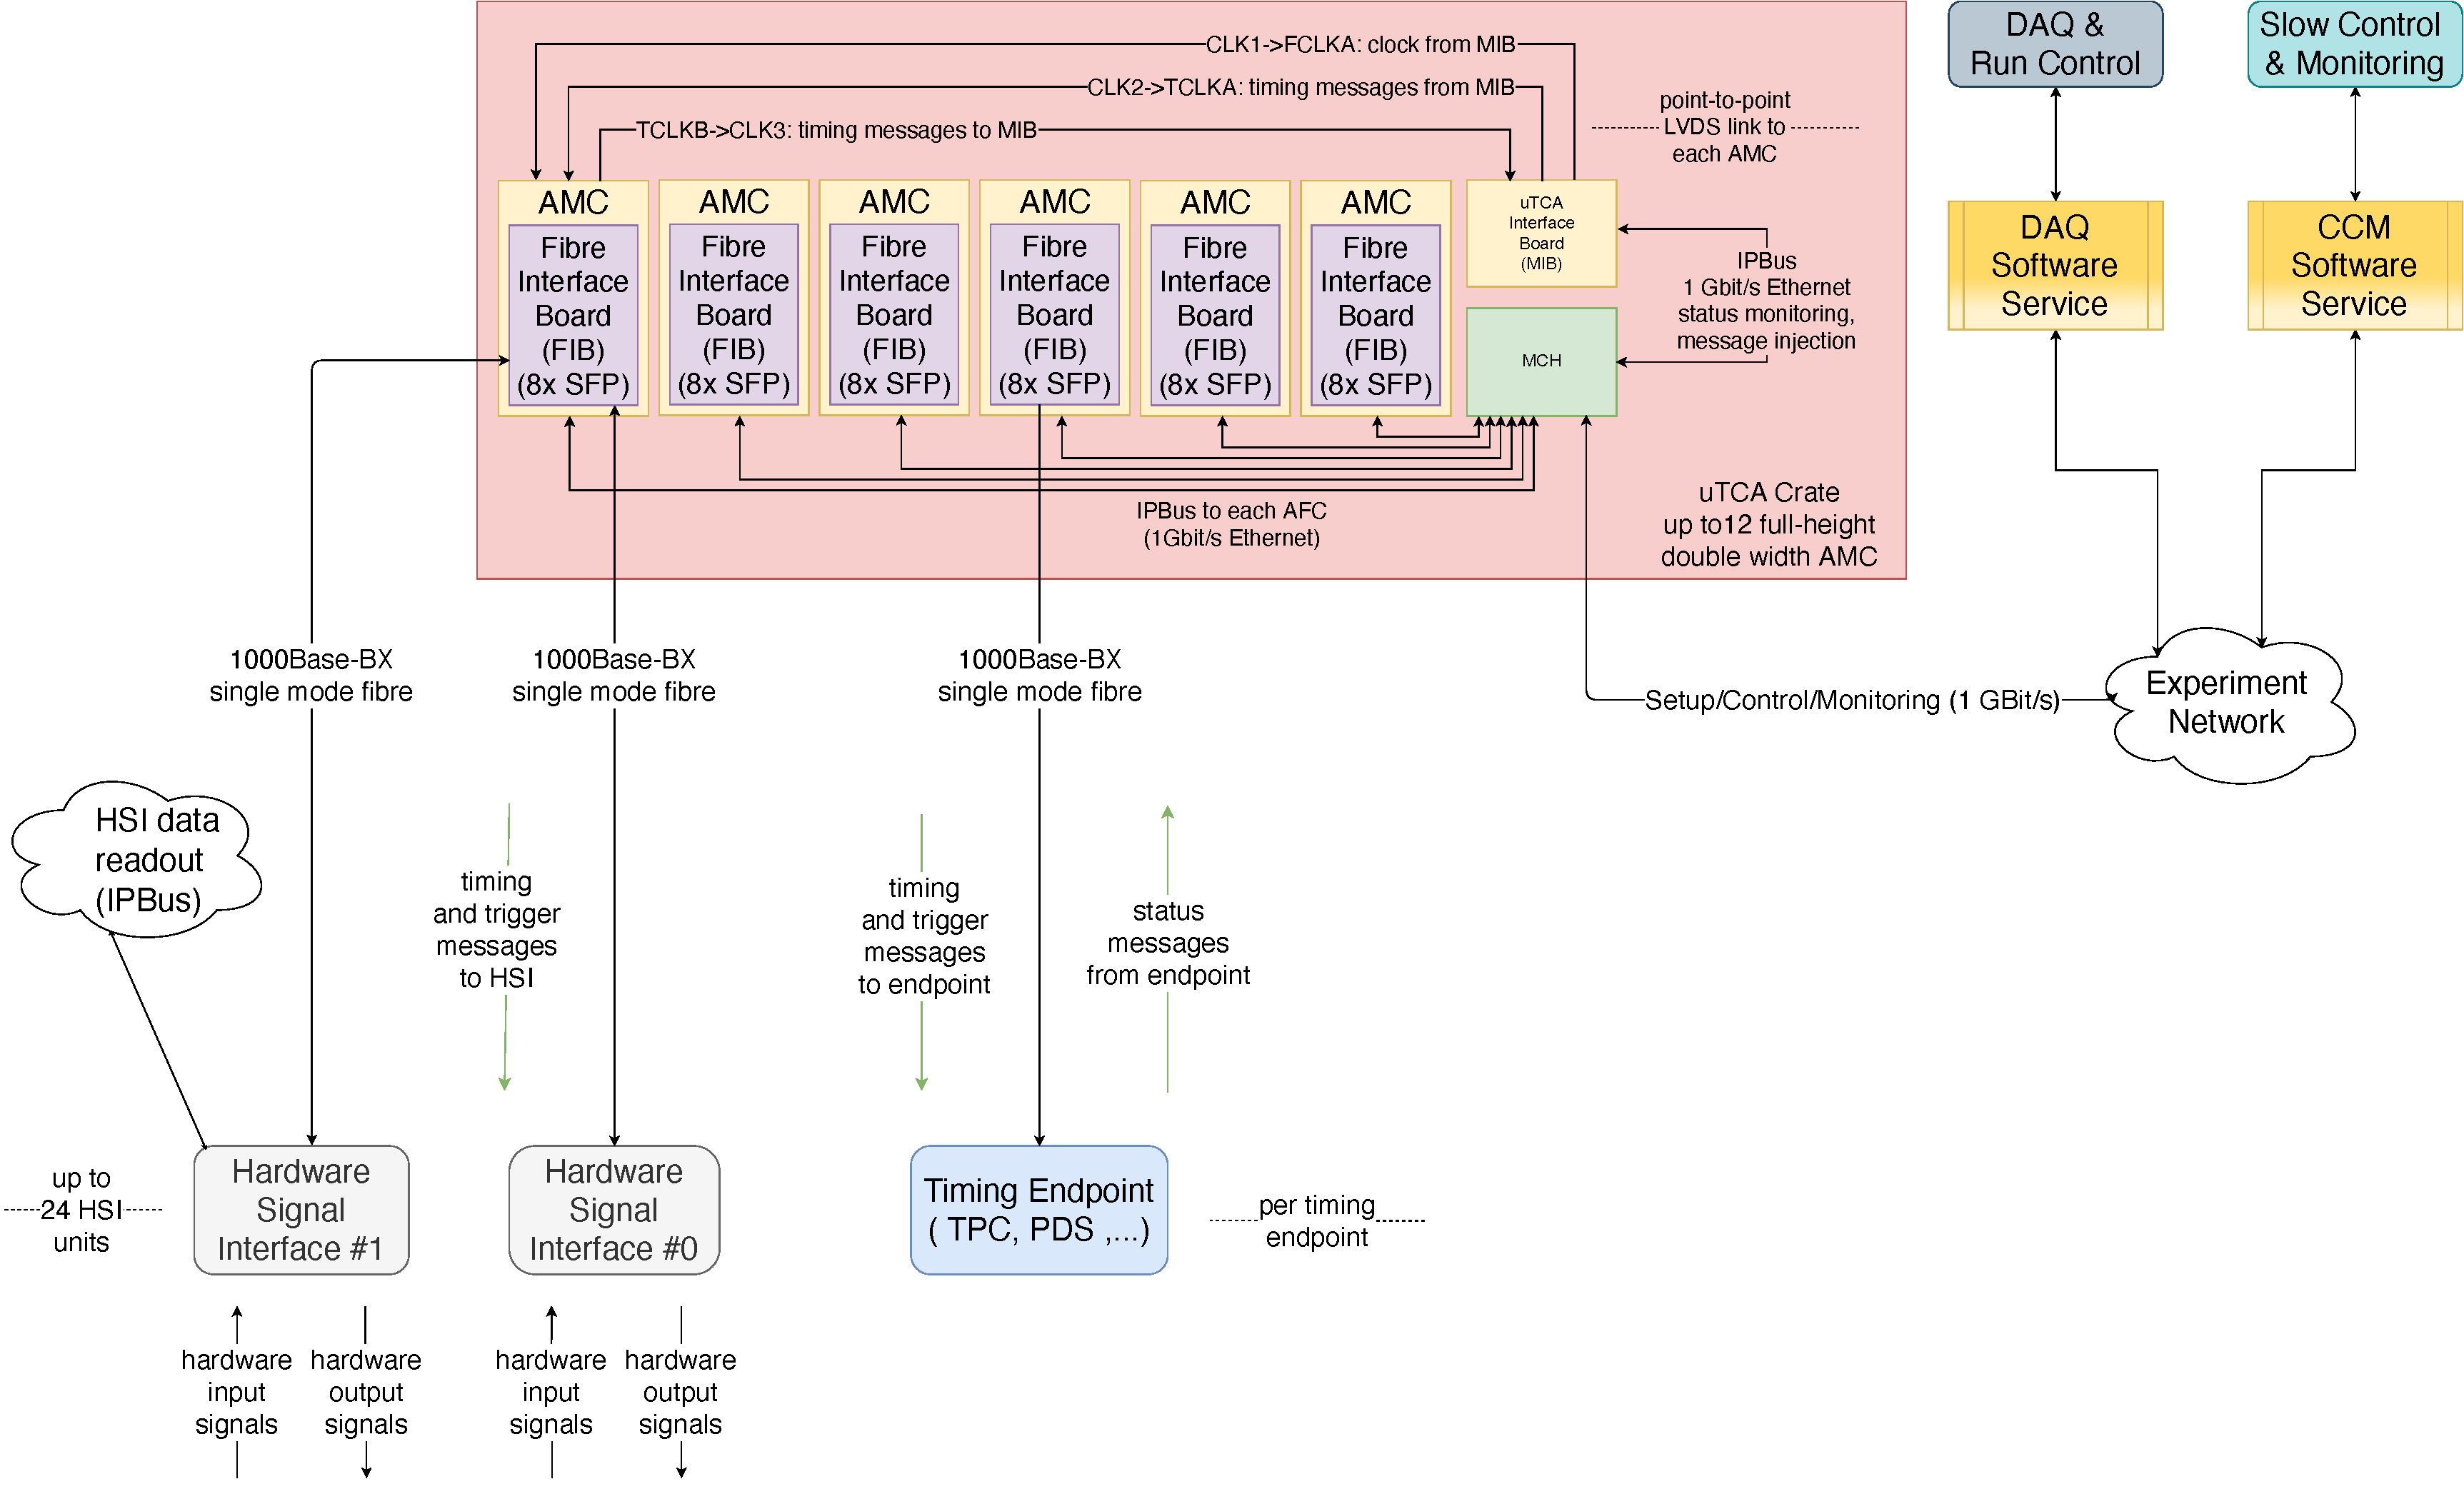
\includegraphics[width=\textwidth]{DUNE_SP_Timing_ETL_interface_1apr20.pdf}
\caption{An illustration of the connections between \dword{mib} and \dwords{amc} inside the \dword{utca} crate, as well as the connections to the \dword{hsi}.}
\label{fig:mib_utca_connections}
\end{figure}
The \dword{mib} has the following functions:

\begin{itemize}
	\item Reception of external timing and command signals
	\item Logging and time-stamping of signals received, distributed or throttled, and transmission to DAQ
	\item Serialisation of timing commands and transmission to the timing network
	\item Phase measurement of incoming timing signals from slaves, i.e. \dwords{fib} and timing endpoints, allowing phase adjustment under software control
	\item Transmission of arbitrary commands and control data under software control
\end{itemize}

The reception of external signals will be achieved using the return data path from the \dword{hsi}, via a dedicated timing endpoint, connected to a \dword{fib} \dword{sfp}. The external signals will be timestamped onto \dword{dts} time domain by the \dword{hsi} endpoint. The external signal \dword{dts} message will then be sent from the endpoint, to the \dword{mib}, via a \dword{fib}. Depending on the type of external signal message, the \dword{mib} may redistribute it to all timing endpoints, or take another action. 
%As well as timestamping external signals onto the \dword{dts} time domain, the \dword{mib} will do the same for \dword{wr} synchronization signals from the \dword{dp} \dword{detmodule}. Reciprocally, \dword{dts} synchronization signals will be timestamped onto the \dword{dp} clock domain. This allows the timing in the \dword{sp} and \dword{dp} \dwords{detmodule} to be aligned. A similar scheme is used to relate the \dword{dts} timing domain to the beam instrumentation \dword{wr} time domain.

To allow timing commands to take effect at all endpoints simultaneously, the delay between the command source, i.e.\ \dword{mib}, and each endpoint, must be measured and compensated for. To achieve this, both the \dword{mib}-\dword{fib}, and \dword{fib}-endpoint delays, must be ascertained.

\subsection{Fibre Interface Board and its carrier}
The \dword{fib}, together with its carrier (an \dword{amc}), act as an active fanout for the \dword{dts} clock and data stream. The clock delivered to the \dword{amc} over the \dword{utca} backplane is routed to the \dword{fib}, where it is fed into a high performance clock generator IC, generating a low jitter version of the clock. The incoming data is routed to the \dword{amc} FPGA, where it is decoded and also fanned out to the eight \dword{sfp} modules on the \dword{fib}. As before, the \dword{dts} data is re-clocked on the low jitter version of the \SI{250}{\MHz} clock using a D-type flip-flop, before it is sent out. The \dword{fib} is connected to its \dword{amc} carrier via an \dword{fmc} connector.

As well as transmitting timing data, the eight \dword{sfp} modules are used to receive timing data from the endpoints. The return data path is used for delay measurements, endpoint status monitoring, and the reception of external signals. The return data path from the eight \dword{sfp} goes via an 8:1 differential multiplexer controlled by the \dword{amc} FPGA, where the expected active \dword{sfp} is the enabled one. Four of the \dwords{sfp} also have a direct connection to the \dword{amc} FPGA allowing external timing signals to enter the \dword{dts}, via the dedicated external signals endpoint, at any time.

The output of the \dword{sfp} modules is connected to an 1:4 passive optical splitter/combiner, allowing each \dword{sfp} to service two \dwords{apa}, assuming two fibres per \dword{apa}. The fact that multiple endpoints are connected to one \dword{sfp} means that only one endpoint can send \dword{dts} data at a time. The endpoint receiving the external triggers will not be connected to an optical splitter/combiner. A block diagram of the components of the \dword{fib} is shown in figure \ref{fig:fib_and_carrier_layout}.

\begin{figure}[h]
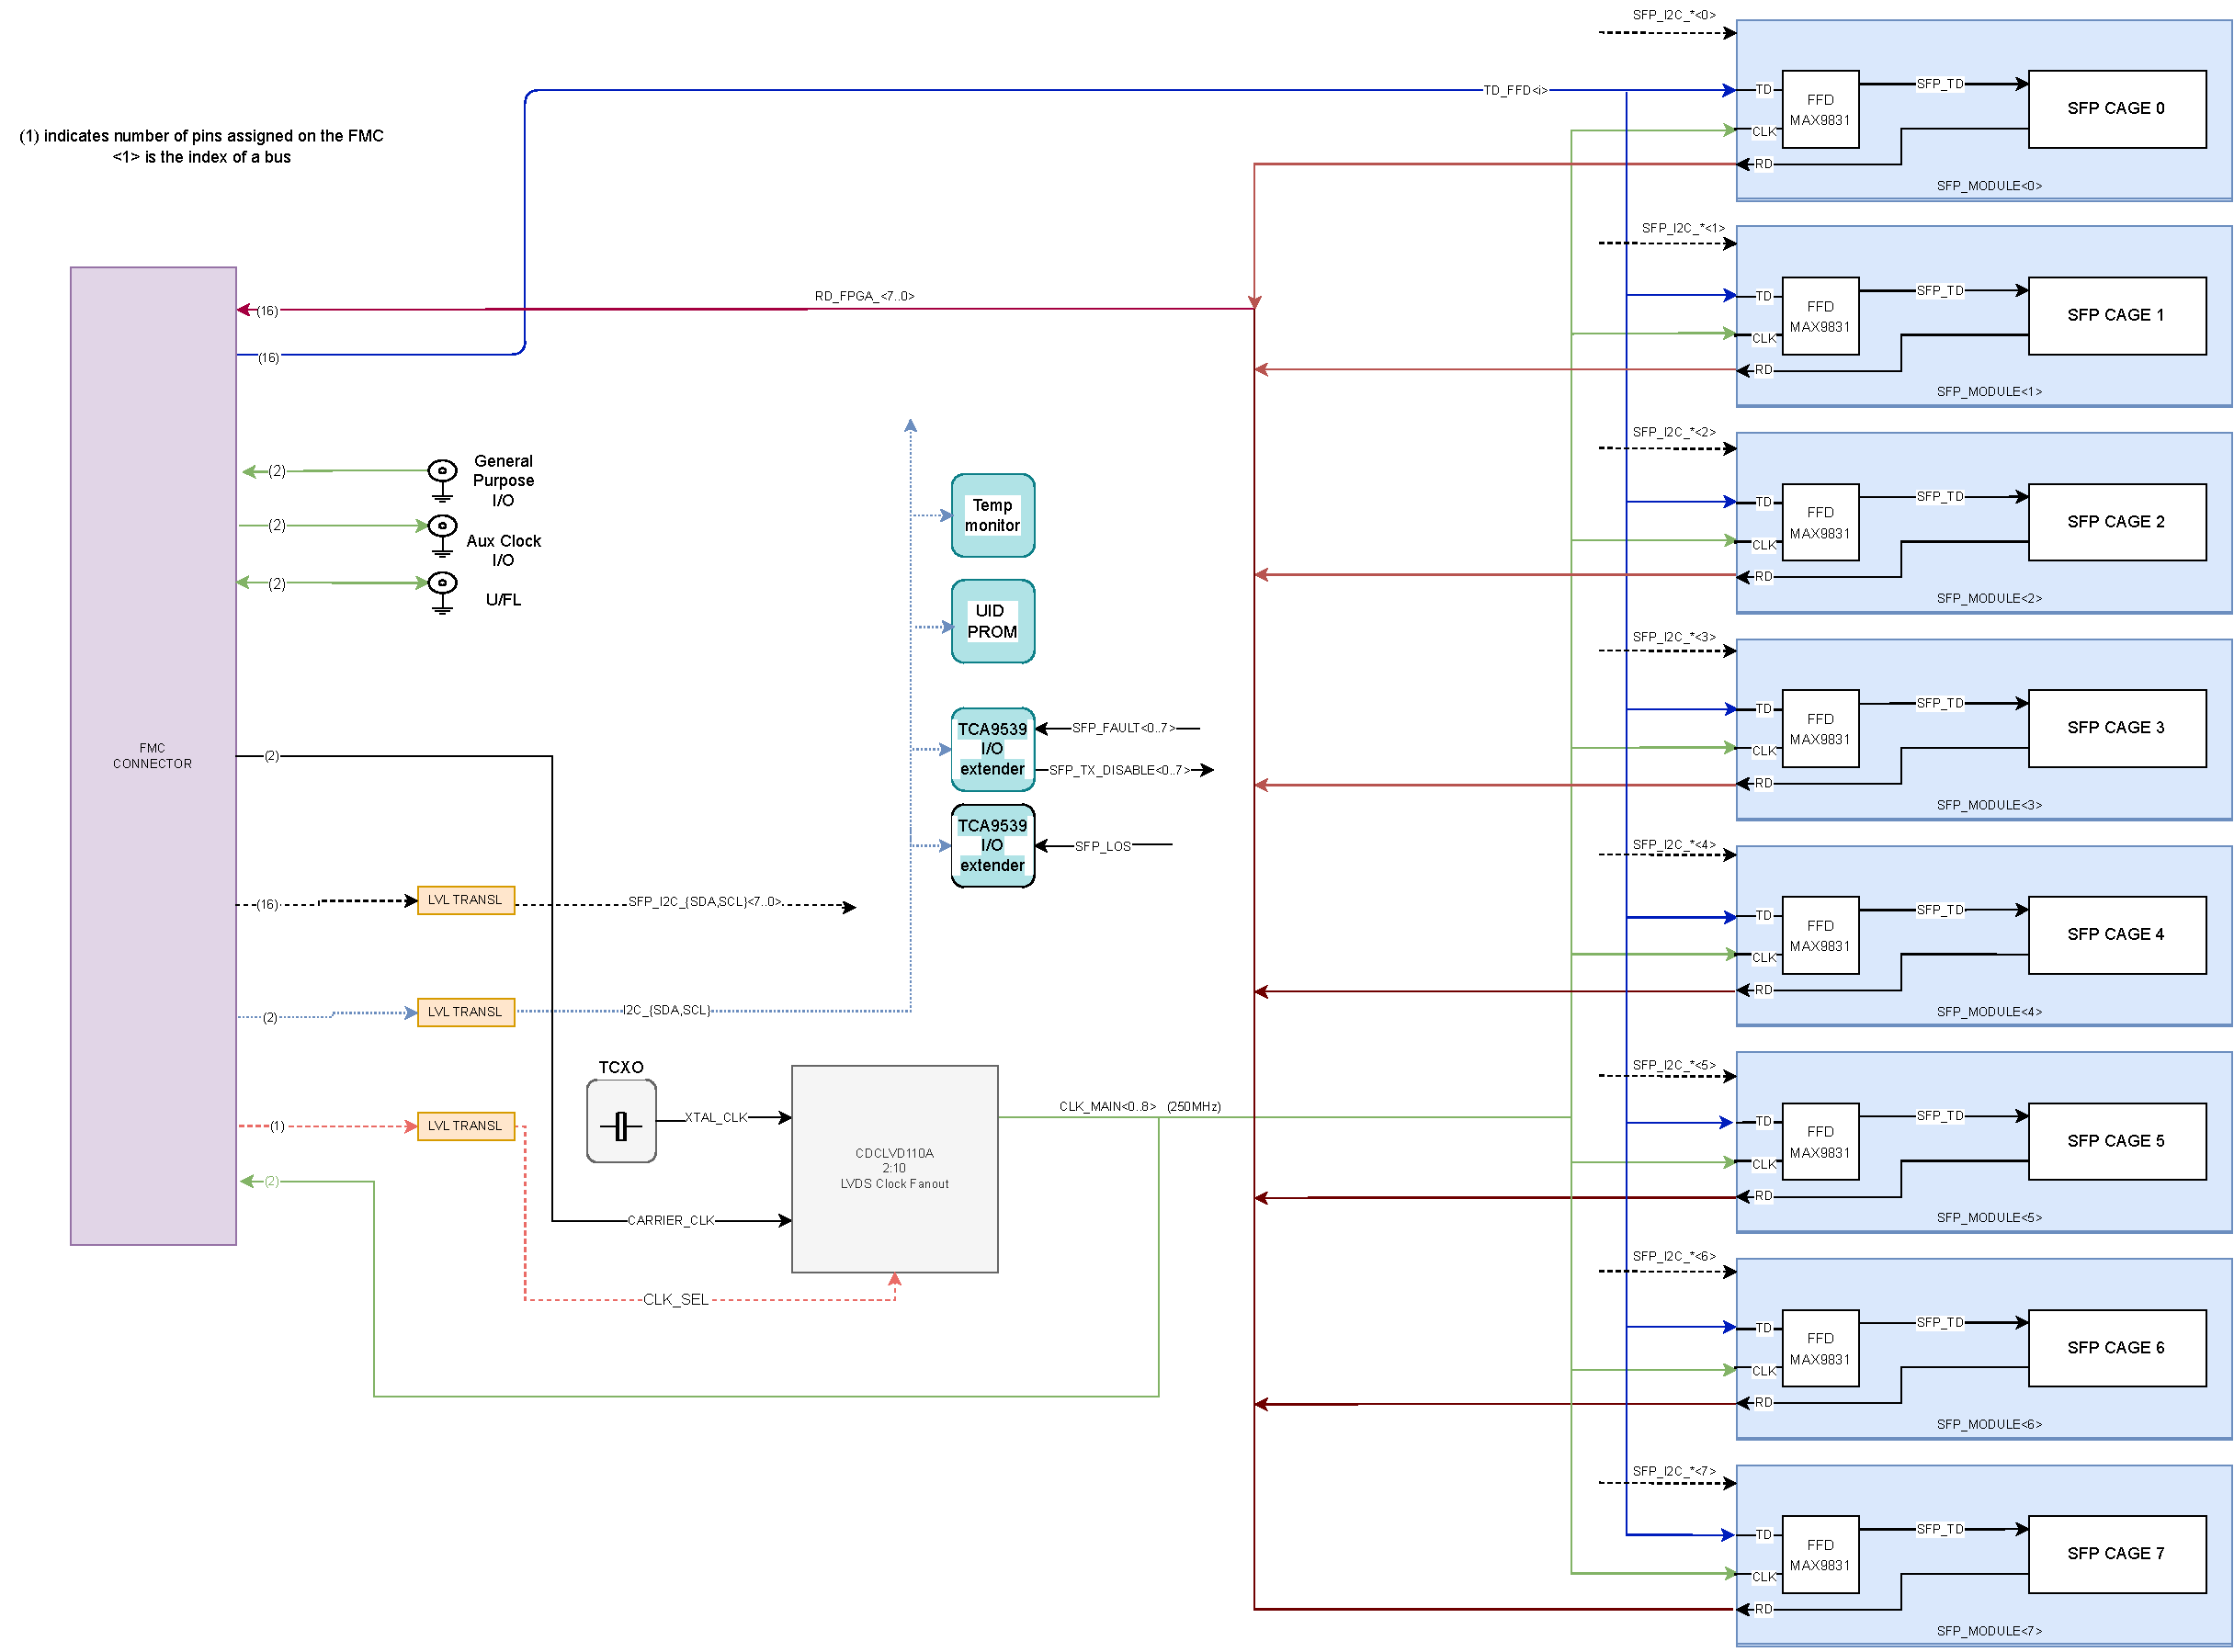
\includegraphics[width=\textwidth]{dune_fib_v2_pc072a.drawio.pdf}
\caption{An illustration of the \dword{fib} components.}
\label{fig:fib_and_carrier_layout}
\end{figure}

The \dword{fib} carrier is envisaged to be off-the-self \dword{amc}. The ohwr.org hosted \dword{afc} design \cite{amc_ohwr}, is currently being evaluated as a potential candidate. The \dword{fib} is a development of a series of timing \dword{fmc} used in ProtoDUNE-SP I. These \dwords{fmc} also served as a ``reference hardware design'' that could be used by groups integrating a \dword{dts} endpoint in their system. A photo of a reference design timing FMC, a \dword{fib} and a \dword{fib} mounted on an \dword{afc} are shown in figures \ref{fig:timing_fmc}, \ref{fig:fib_photo} and \ref{fig:fib_afc_photo} respectively.

\begin{figure}[h]
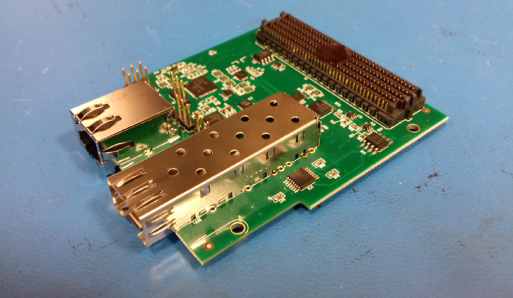
\includegraphics[width=\textwidth]{timing_fmc.pdf}
\caption{A photo of a ``reference design'' FMC.}
\label{fig:timing_fmc}
\end{figure}

\begin{figure}[h]
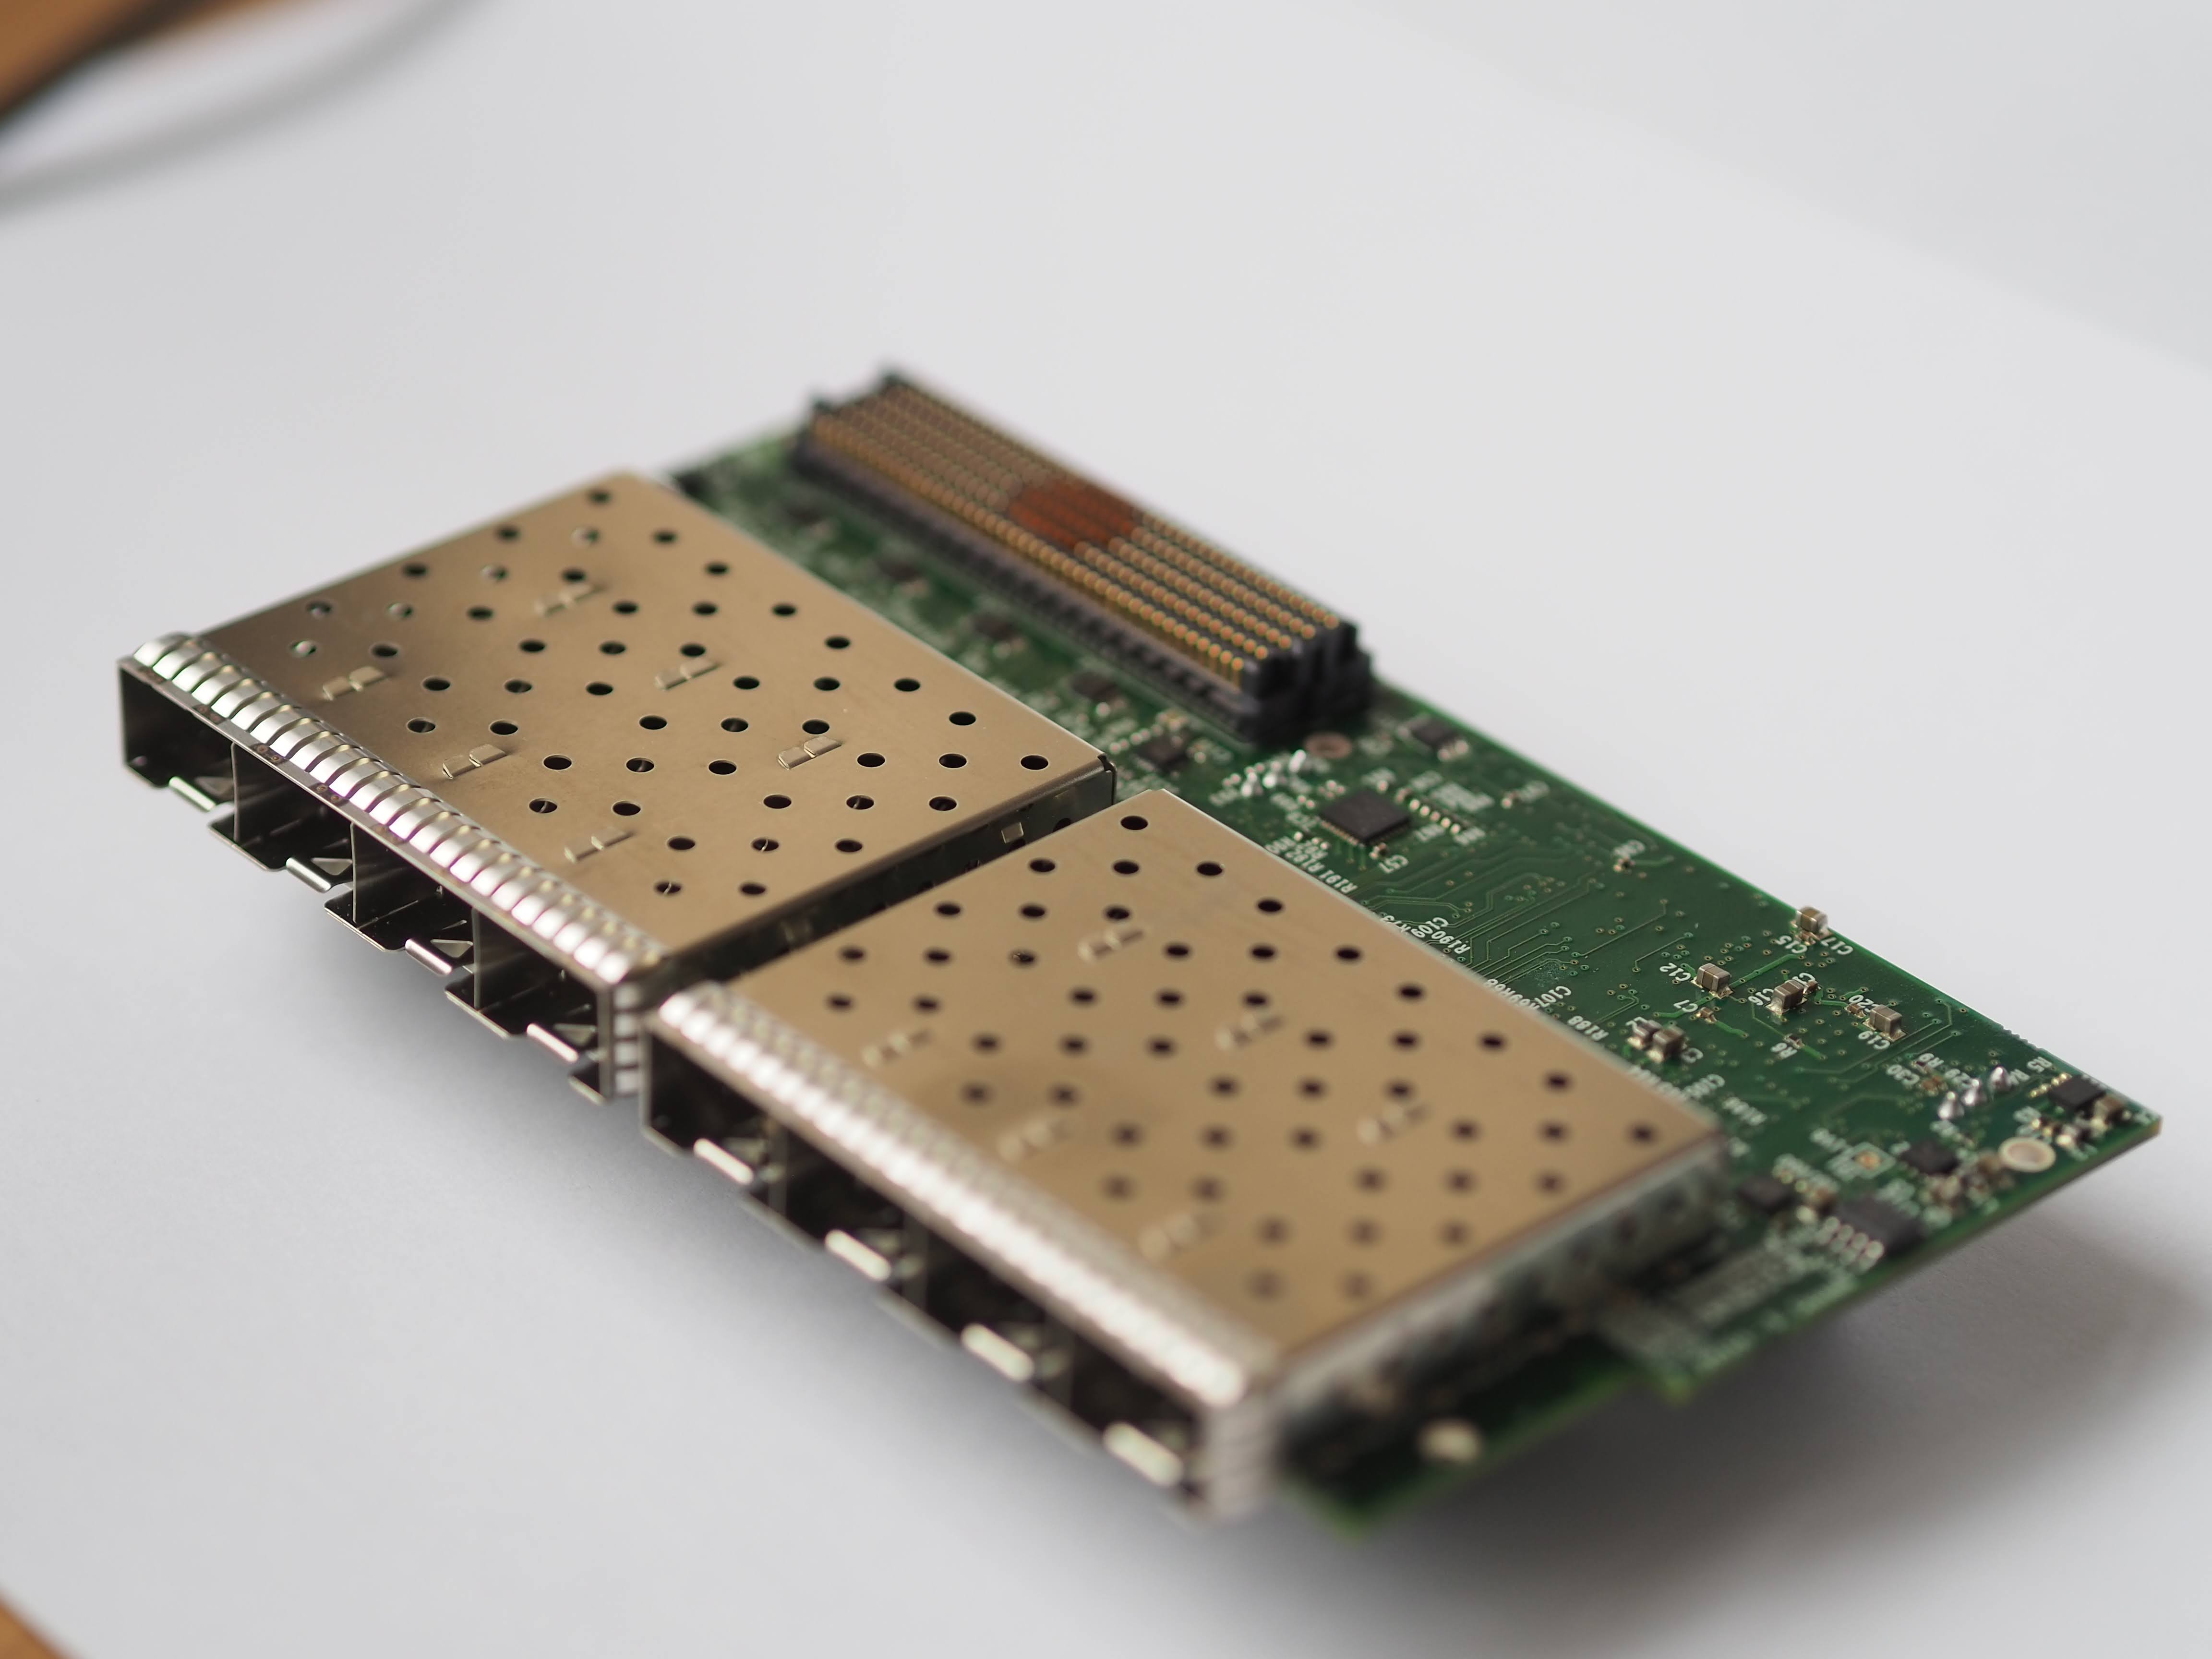
\includegraphics[width=\textwidth]{P7230005.jpg}
\caption{Photograph of a \dword{fib}.}
\label{fig:fib_photo}
\end{figure}

\begin{figure}[h]
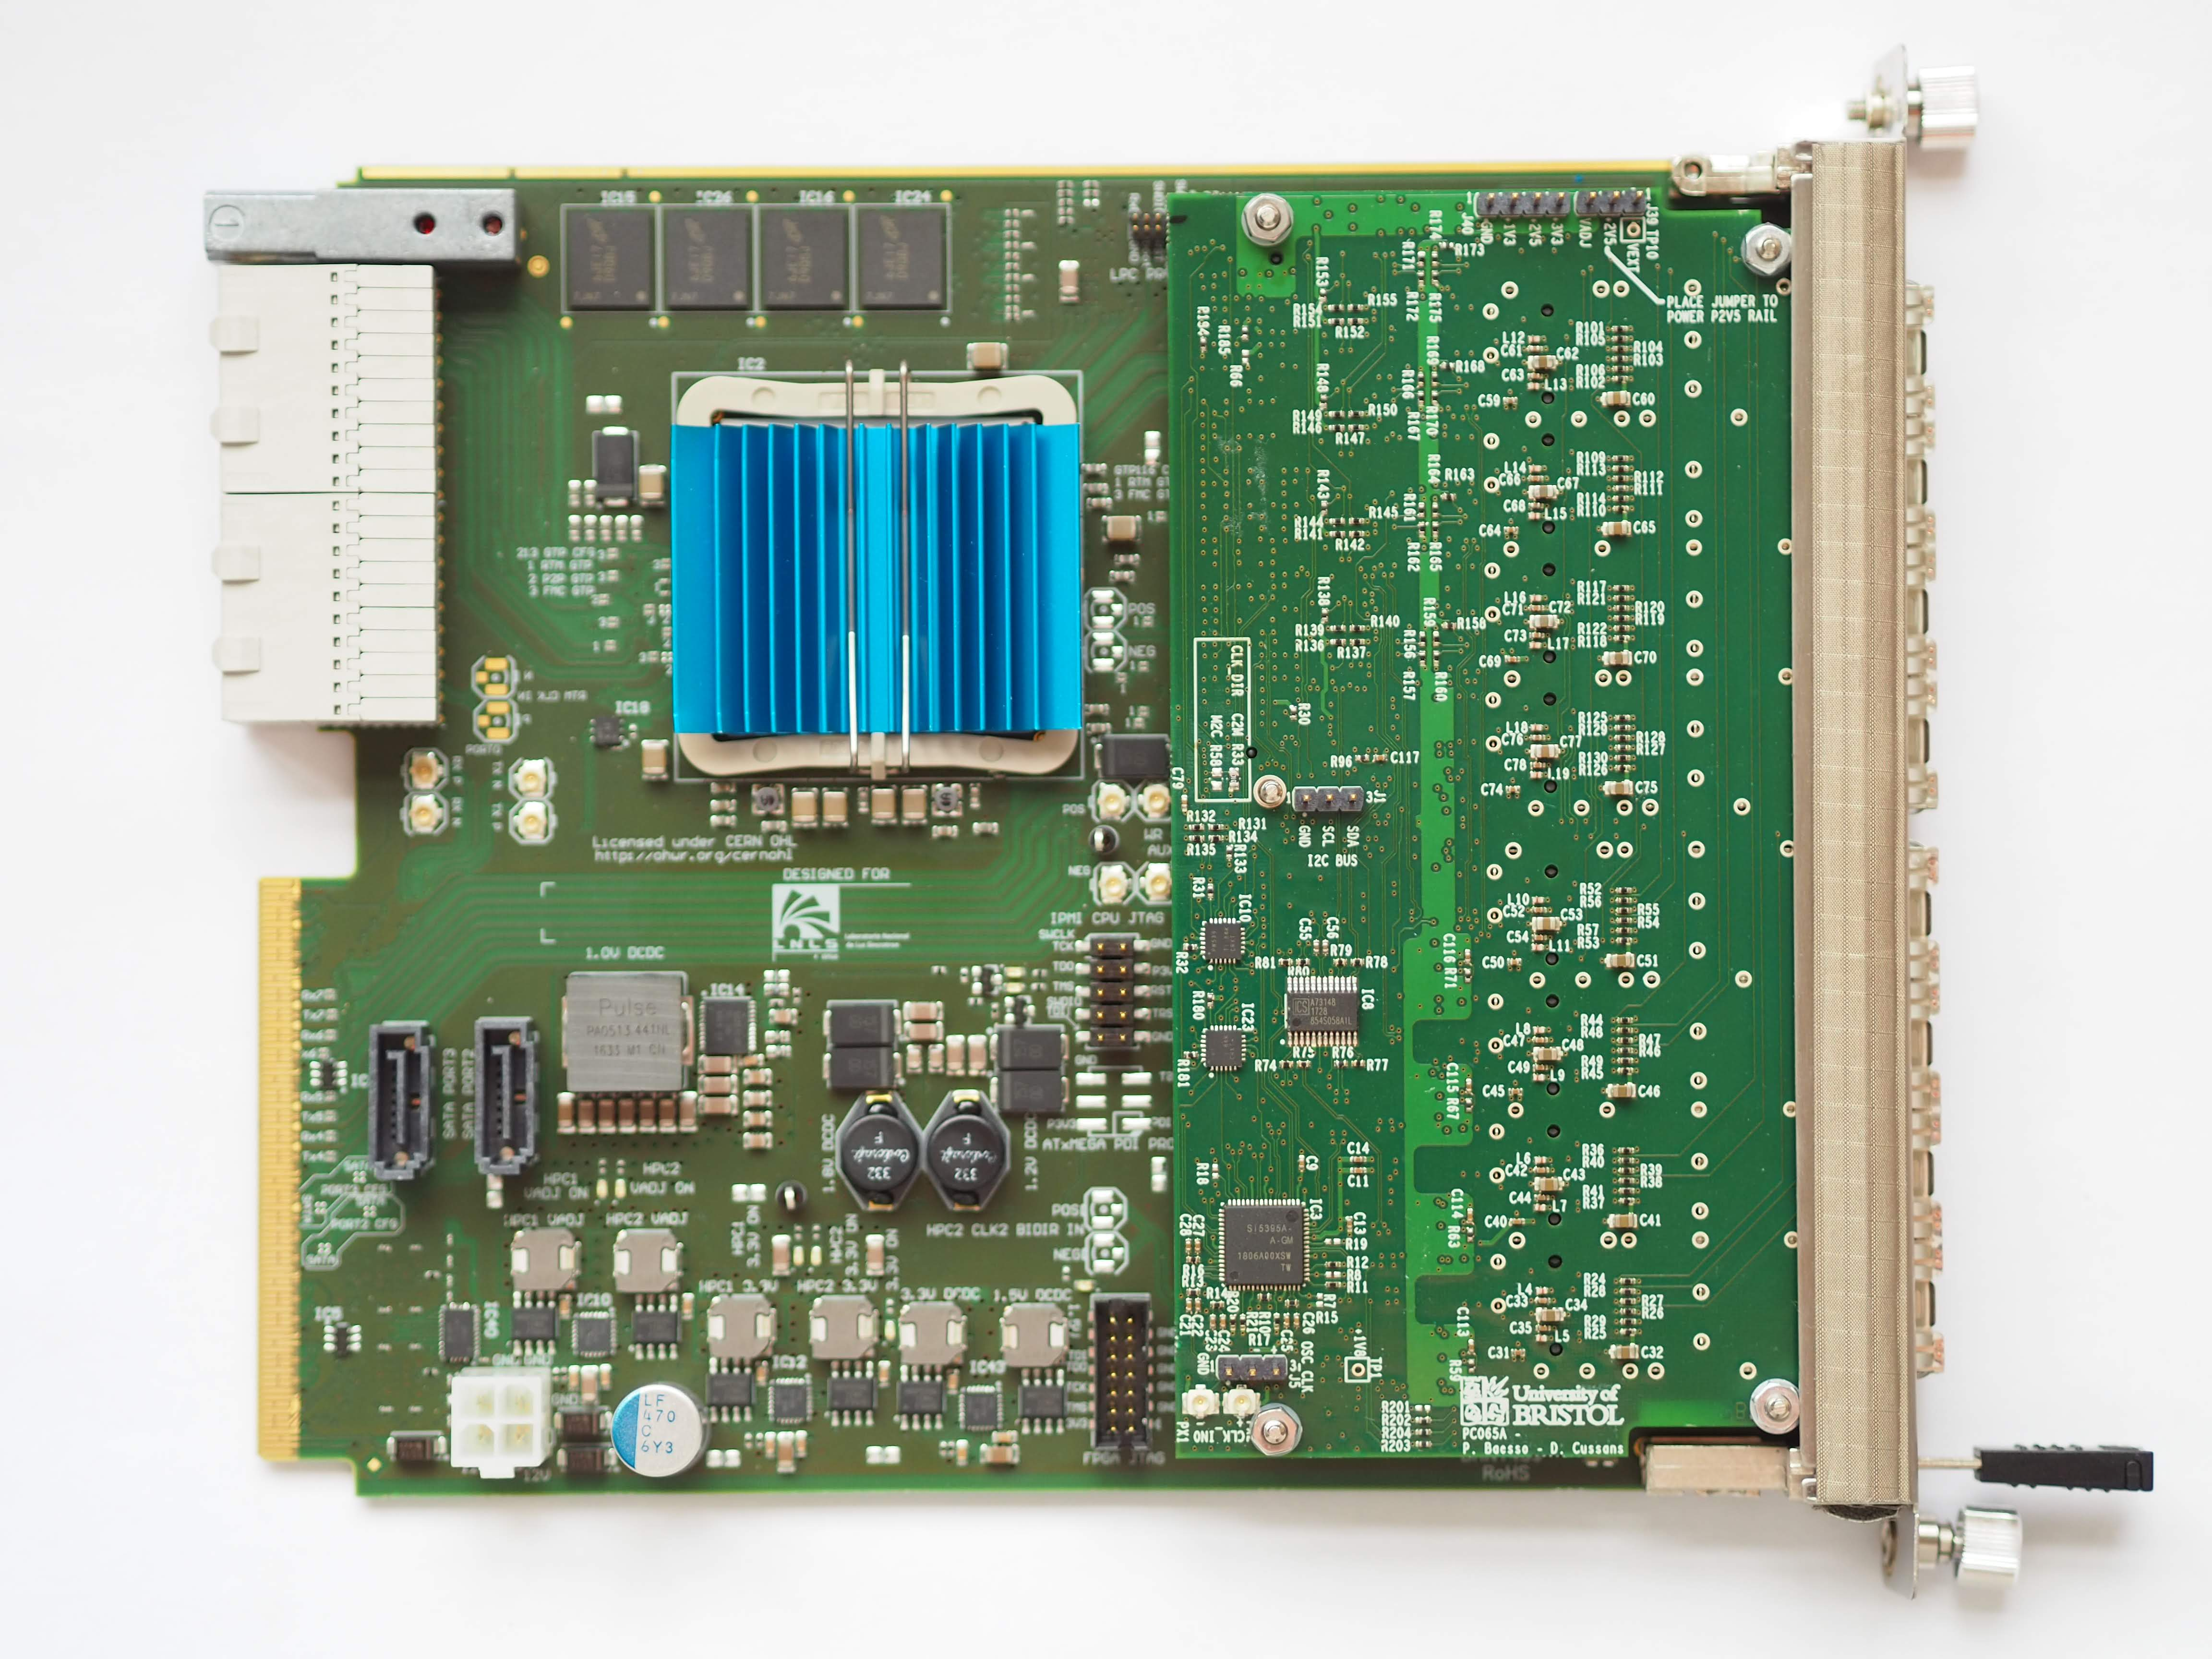
\includegraphics[width=\textwidth]{OI000293.jpg}
\caption{Photograph of a \dword{fib} mounted on an \dword{afc}.}
\label{fig:fib_afc_photo}
\end{figure}

Monitoring and control of each \dword{amc} and its \dword{fib} will be done over GBit/s Ethernet. Two differential lines are used to establish a 1000BASE-X Ethernet connection between the \dwords{amc} and the \dword{mch}.

\subsection{Endpoint}
Endpoints decode the timing signal into separate clock and data
signals using a \dword{cdr} IC, which in turn feeds a low-bandwidth PLL for applications requiring a very low jitter local clock. A common firmware block is used to decode the timing protocol, which is incorporated into the overall firmware design for the receiving FPGA in each DAQ component. This block provides a cycle counter, several independent command and synchronisation signals, and a general-purpose packet data output to each endpoint. The cycle counter may be used further to generate low-frequency timing signals for further propagation, e.g. the \SI{2}{\MHz} sampling signal for the cold ADCs.
\subsection{Redundancy}
The extremely high uptime requirements of the DUNE experiment translate into similarly high uptime requirements on the timing system. The uptime requirements on the timing system exceeds those of the overall experiment due to the fact that the timing system is an essential part of the experiment infrastructure, and no system can operate without it. To facilitate the uptime requirements, the timing system has been designed to include two complete and independent timing chains, where the whole or a part of one system is active, and the other one acts as hot spare.

There are two GPS antennae, one on top of the Yates shaft and another on top of the Ross shaft. Each antennae feeds a GPS receiver and a \dword{gib}, producing two independent \dword{dts} clocks and timestamps. Cross-referencing the two independent signals, potentially against a third signal, e.g. a rubidium oscillator, allows for any drifts or other issues in one of the \dword{dts} timing streams to be detected. At any one time, only one of the \dword{dts} clock and timestamp are actively used.

The two \dword{dts} timing streams are both fed into two \dword{utca} crates. There is one set of two \dword{utca} crates per \dword{spmod}. Each crate is populated with the full timing \dword{utca} payload, i.e. a \dword{mib}, \dword{mch}, and the \dword{amc}+\dword{fib} pairs. The output of the \dword{sfp} modules from the two \dword{utca} crates are brought together into a 2:1 passive optical combiner/splitter. This configuration allows the switching of operation between the two crates to happen without physical intervention. 

The fibres from the 2:1 optical combiner/splitter serving the \dword{hsi} connect directly to the unit. For fibres feeding detector timing endpoints, the output of the 2:1 optical combiner is fed into a 1:4 splitter/combiner, which is used to fan out the \dword{dts} timing stream. The optical connections will use single-mode fibres, and 1000Base-BX-20 \dword{sfp} transceivers, transmitting at 1310 nm and receiving on 1550 nm. Only one endpoint at a time, of the endpoints sharing an \dword{sfp} via the 1:4 splitter, can transmit a return signal.

The design also allows both crates to be partially active. This may be useful in a scenario, where a \dword{fib} in the active crates becomes faulty, and the recovery action would be to enable the equivalent \dword{fib} in the redundant crate. This would isolate the disruption of the timing signal only to the endpoints supplied by the faulty \dword{fib}, rather than the whole \dword{spmod}. It is also possible to use just a single \dword{sfp} module of the redundant crate, minimising disruption to the DUNE data-taking even further.

The arbitration of which \dword{dts} timing stream and physical hardware is providing the timing for the \dword{spmod} will be done by the DUNE \dword{ccm}. The \dword{ccm} system is natural candidate for this role, as it has high-level overview of the whole DUNE detector, including the timing system. The CCM may initiate a hot-swap action, however the responsibility for the actual implementation and execution of the swap mechanism lies in the domain of the timing system.

%Due to different development histories of the \dword{bde} and \dword{tde} technologies of the \dword{vd} \dword{detmodule}, different timing systems are used for each one. The \dword{vd} \dword{bde}, as well as the entirety of the \dword{hd} \dword{detmodule} make use of the \dword{dts}. The protocol is based around a 8b/10b encoded serial data stream, and it distributes a \SI{62.5}{\MHz} clock to \dword{hd} and \dword{vd} \dword{bde} endpoints. The \dword{vd} \dword{tde} are synchronised via a \dword{wr} network \cite{wr_ohwr}, which uses a \SI{125}{\MHz} clock. The \dword{wrgm} of the \dword{vd} \dword{tde} \dword{wr} network will be driven by a \SI{10}{\MHz} clock and \dword{pps} provided by a specialised \dword{dts} endpoint.

%%%%%%%%%%%%%%%%%%%%%%%%%%%%%%%%%%%%%%%%%%%%%%%%%%%%%%%%%%%%%%%%%%%%%%%%%%%%%%%%%%%%%%%%%5
\subsection{Timing Distribution Within Readout Systems}

In general the timing and synchronization signals from the \dword{dts} endpoint are distributed inside the readout system using a mechanism that depends on the readout system. In all cases any latency introduced by clock/timing distribution inside the readout system should be compensated for in the data returned to the DAQ.

\subsection{Horizontal Drift TPC readout and Vertical Drift TPC bottom electronics}


For the \dword{hd} drift readout electronics and VD bottom drift electronics a single fibre is connected to each \dword{wiec} and timing signals are distributed to DTS endpoints in the \dwords{wib}. Clock and data are then transmitted in custom protocol to the \dwords{femb}

\subsection{Vertical Drift TPC top electronics}

For the \dword{vd} top drift electronics a special \dword{dts} endpoint produces 10MHz clock and 1 pulse per second signals, locked to the \dword{dts} master clock. These are then used to synchronize a \dword{wr} system\cite{wr_ohwr} which distributes timing information to the ADC boards.

\section{Monitoring}
Monitoring is an essential function of the \dword{dts}, and will be key in enabling DUNE to meet its uptime requirements. To this purpose, comprehensive and and coherent monitoring information from the whole \dword{dts} must be made available to the DUNE \dword{ccm}.

\subsection{Endpoint monitoring}
Timing endpoints are monitored through two separate pathways. The \dword{dts} itself periodically interrogates each endpoint, using the \dword{dts} protocol, and report its status to the \dword{ccm}. The other monitoring pathway is composed of the timing endpoint itself interacting with the \dword{ccm}. Parameters which will be monitored include:

\begin{itemize}
  \item timestamp synchronisation
  \item clock frequency, relative to the endpoint free-running oscillator
  \item endpoint state
  \item command counters
  \item measured endpoint calibration parameters, e.g. delay path.
\end{itemize}

\subsection{System monitoring}
As well as its endpoint, the \dword{dts} will monitor its own functions and status, and report the results to \dword{ccm}. This information will be vital in enabling the hot-swap functionality of the system. Some of the parameters which will be monitored for different \dword{dts} components are:

\begin{itemize}
    \item \dword{gpsdo} receiver: strength of signal, list of satellites visible. 
    \item \dword{gib}: time code provided by \dword{gpsdo} receiver, link to \dword{mib}, \dword{dts} timestamp-\dword{utc} relationship.
    \item \dword{utca} crate: temperature, supply voltages, power consumption, fan speed.
    \item \dword{mib}: frequency of recovered clock (relative to a free-running oscillator), power voltages and current, board temperature, command counters/rates, clock chip status, link to \dword{gib}, relative timestamp and clock phase between two upstream \dwords{gib} .
    \item \dword{fib}: status of each \dword{sfp} module, frequency of received clock (relative to a free-running oscillator), clock chip status, board temperature, link to \dword{mib}.
    \item \dword{sfp}: Tx/Rx optical power, temperature, supply voltage, laser current.  
\end{itemize}

\subsection{Software API}
Communication between the \dword{dts} and the \dword{ccm} will be realised through a software interface. This software layer will implemented the low level functions required to send and receive information between the itself and the \dword{dts}, e.g. the reading and writing of \dword{mib} firmware registers using IPBus \cite{ipbus}. These low-level command will be used to construct the higher-level functions, e.g. reporting of \dword{mib} status, or endpoint reset. The software API will then expose these higher level functions to the \dword{ccm}.

%\section{Design and system validation}
%The development and validation of the \dword{dts} is based around iterative incremental model, where the functionality of the system is built up step-by-step. As per the overall DUNE development strategy, each system or technology  which will be used in the eventual DUNE \dword{fd} must first be demonstrated to be fit for purpose at the ProtoDUNE experiments at CERN. The timing system is no different, and has fully embraced this ethos. Two distinct \dword{dts} prototypes will be used for the two phases of the ProtoDUNE SP experiment. The use of the \dword{dts} at the ProtoDUNE experiments will be especially useful in validating the operational requirements, external system interfaces, and long-term stability of the system. The validation of the \dword{dts} system will also heavily rely on test and measurements performed in a laboratory environment, e.g. alignment of timing endpoints to within \SI{1}{ns}. 

%\subsection{Tests at ProtoDUNE-SP I}
%A prototype of the \dword{dts} was developed and successfully used to synchronise the components of ProtoDUNE SP I. The system uses an AIDA 2020 TLU as a master unit, which receives external signals from the trigger system and SPS accelerator, as well as a high-quality \SI{10}{\MHz} reference, which is used to generate the ProtoDUNE SP I \SI{50}{\MHz} clock. The master unit also multiplexes synchronization and trigger commands, along with arbitrary command sequences generated by software, into a single encoded data stream. The timing data stream is fanned out to the endpoints via the means of an active fanout module and single-mode fibres. At each endpoint, a commercial \dword{cdr} device is used to recover separate clock and data signal from the data stream, which are used to synchronise the endpoint.

%The system operated successfully for the duration of the data-taking and has demonstrated the following functionalities:

%\begin{itemize}
%    \item generation and distribution of a stable master clock to DAQ components
%    \item timestamping of external signals onto the ProtoDUNE SP I time domain
%    \item distribution of synchronisation, trigger and calibration commands to the DAQ system.
%\end{itemize}

%These functionalities form a core part of the expected role of the \dword{dts}, however certain other key aspects of the system were not tested at ProtoDUNE SP I. Some of these include:

%\begin{itemize}
%    \item GPS interface and IRIG decoding
%    \item Synchronisation with UTC
%    \item Synchronisation between endpoints
%    \item \dword{utca} fanout hardware.
%\end{itemize}

%The issues listed above will be addressed by the prototype developed for ProtoDUNE SP II, as well as prototype testing in a laboratory.

%\subsection{Tests at ProtoDUNE-SP II}
%The ProtoDUNE-SP I timing system demonstrated several key functions of the eventual \dword{dts}, however the hardware used to construct the prototype is not aligned with that of the actual DUNE \dword{dts}. This issue be remedied by the ProtoDUNE-SP II prototype, which will use the full chain hardware components described in section \ref{sec:system_design}, i.e. from GPS receiver to timing endpoint. This second prototype will also be used to test synchronisation between endpoints and UTC. The validation of these requirements will be done both at ProtoDUNE SP II and in the laboratory. The frequency of the system clock will be increased to the expected \dword{dts} value of \SI{62.5}{\MHz}.

%Another advantage of deploying timing system prototypes at the ProtoDUNE experiments is that it allows the assessment of the long-term stability of the system, and associated operational challenges. This type of long-term operation feeds directly into the validation of the uptime requirements of the final \dword{dts}.

%\subsection{Tests in laboratory}
%For ProtoDUNE SP II, it is not envisaged that a fully redundant system will be deployed, however the functionalities associated with having two independent timing chains must still be developed and tested. Most of this work will be carried out in a laboratory setting, with a representative setup of the \dword{dts}. Laboratory tests will also be needed to carry out disruptive tests, such as endpoint or system wide fault recovery and firmware development.

%\section{Commissioning}
%The \dword{dts} will be one of the first DAQ components installed, so that timing and synchronization signals are available the other components of the DAQ as soon as they start to be installed. Early in the construction project \dword{spts} ``development kits'' will be made available. The kits will include the hardware and software needed to produce \dword{spts} timing signal. This will allow the teams developing the DUNE readout systems to integrate with the \dword{spts} early in the development process. Hardware and software will also be available for use in vertical slice tests and the \dword{itf}. 

\end{document}